\Chapter{Related Work}\label{chapter:related}

In this chapter, I provide a comprehensive review of existing
approaches relevant to multi-view image generation.

The chapter begins by introducing the fundamental task of Novel View
Synthesis (NVS) and its significance. We then delve into traditional
3D reconstruction techniques (Section \ref{sec:3d-reconstruction})
and their inherent limitations, particularly for sparse-input
scenarios, which motivates the exploration of generative methods.
Subsequently, the discussion shifts to the foundational principles of
Deep Generative Models for Image Synthesis, with a focus on diffusion
models (Section \ref{sec:text-to-image}).

Building on this, we explore various methods for Conditioning
Diffusion Models for Enhanced Control and New Tasks (Section
\ref{sec:conditioning-diffusion}), including the crucial role of
camera parameter encoding and the concept of lightweight adaptation
through adapters.

The core of the chapter then examines state-of-the-art
Diffusion-based Multi-View Image Generation techniques (Section
\ref{sec:multi-view-diffusion}), covering both single reference image
novel view synthesis and architectures for coherent multi-view
generation, including specialized multi-view adapters.
%  Finally, the chapter will conclude with a summary of the discussed
% methods and highlight identified research gaps that this thesis
% aims to address.

\section{Traditional 3D Reconstruction Approaches}\label{sec:3d-reconstruction}

Simultaneous Localization and Mapping (SLAM) is a fundamental concept
in the field of computer vision and robotics. It refers to the
process of simultaneously estimating the camera's position and
orientation in a 3D environment while mapping the environment itself.
Originally, SLAM was used to track the position of a robot in a 3D
space, but it has since been applied to a wide range of problems,
including augmented reality, medical applications and novel view
synthesis.

SLAM works by processing sensor data in real-time to create a map of the unknown environment while simultaneously tracking the position of the sensor within that map. This process typically involves several key steps:
\begin{enumerate}
  \item \textbf{Feature Detection}: Identifying distinctive points or features in the environment from sensor data
  \item \textbf{Data Association}: Matching observed features with previously mapped features
  \item \textbf{State Estimation}: Updating the estimated pose of the camera and the map of the environment
  \item \textbf{Loop Closure}: Recognizing when the sensor has returned to a previously visited location and adjusting the map accordingly to reduce accumulated errors
\end{enumerate}

To address these requirements, researchers have
concentrated on creating techniques for machines to independently
build ever more precise scene representations. This integration of
robotics, computer vision, sensor technology, and recent advancements
in artificial intelligence has shaped this field.

Typically, SLAM techniques use a combination of data sources, such as
images, laser range scans, sonars and GPS to effectively map an environment.
In this work I will focus on the use of images for 3D reconstruction.

\subsection{Structure from Motion Pipeline}

One of the most popular methods for 3D reconstruction from images is
COLMAP \cite{colmap}. COLMAP is a general-purpose
structure-from-motion (SfM) \cite{multipleviewgeometry} system that
can automatically reconstruct 3D scenes from a collection of images.
It is a popular choice for 3D reconstruction due to its accuracy,
speed, and ease of use.

\begin{figure}[h]
  \centering
  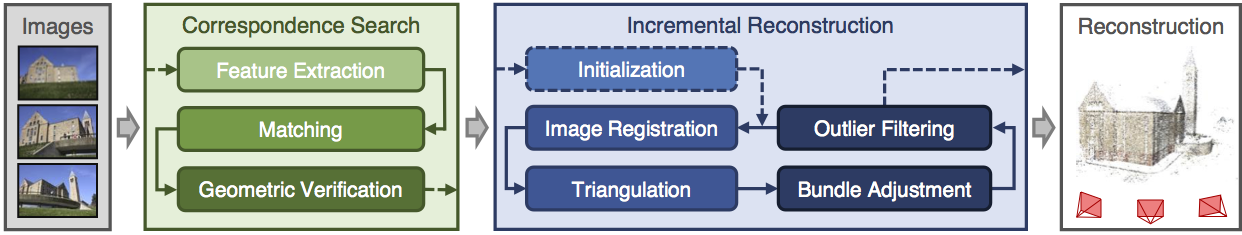
\includegraphics[width=0.9\textwidth]{images/related-work/COLMAP.png}
  \caption{COLMAP pipeline}
  \label{fig:colmap-pipeline}
  % https://colmap.github.io/tutorial.html
\end{figure}

Structure from Motion works in two main steps [Figure
\ref{fig:colmap-pipeline}]:
\begin{enumerate}
  \item \textbf{Correspondence Search}: Identify the unique landmarks
    (features) in all of the images and match the same landmarks across images.
  \item \textbf{Incremental Reconstruction}: Estimates the camera
    poses and triangulates 3D points through an iterative process.
\end{enumerate}

First step of correspondence search is feature extraction. COLMAP
uses SIFT \cite{sift} and ORB \cite{orb} methods to extract features
from images. Scale-invariant feature transform (SIFT) is a method for
detecting keypoints that contrast with their surroundings and
describing the local image content around them. It is invariant to
rotation and scale, making it robust for matching features across images taken from different viewpoints and distances. Oriented FAST and Rotated BRIEF (ORB) is a more
computationally efficient alternative to SIFT, combining a high-speed
FAST detector with optimized descriptors for rotation invariance,
offering comparable matching performance with significantly reduced computational requirements.

\begin{figure}[h]
  \centering
  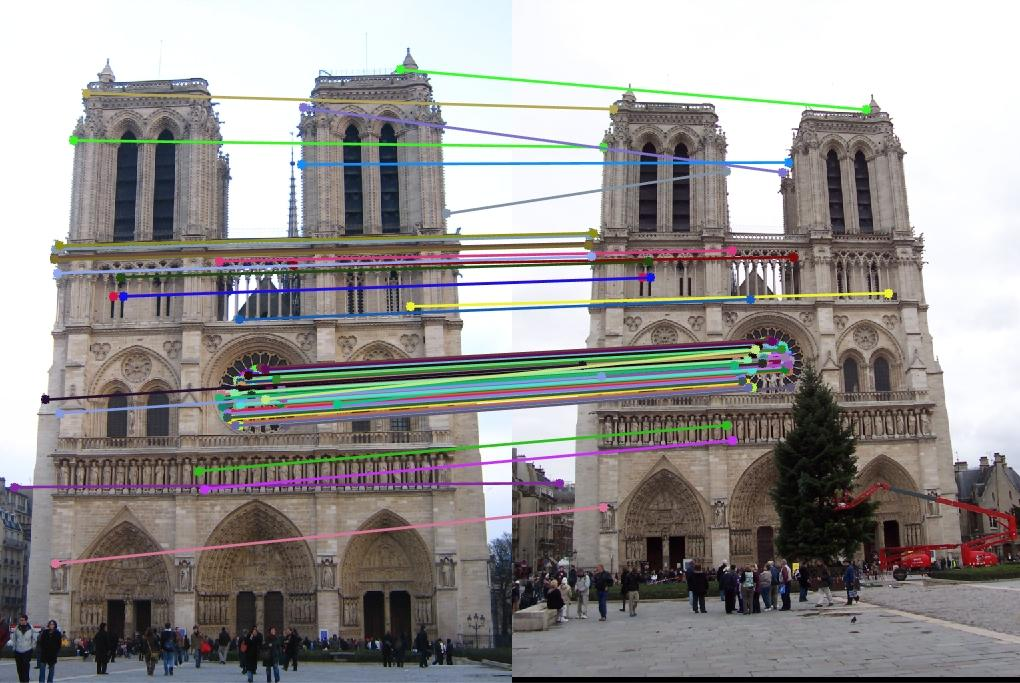
\includegraphics[width=0.7\textwidth]{images/related-work/feature-matching.jpg}
  \caption{Feature matching result}
  \label{fig:matching-features}
  % https://blog.roboflow.com/image-matching/
\end{figure}

Second step is matching features across images. Feature matching is a
process of finding the best matches of features across the images.
COLMAP uses a variant of the FLANN \cite{flann} library to find the
best matches for each feature. FLANN is a library for performing fast
approximate nearest neighbor searches in high dimensional spaces.
Feature matching is visualized in Figure \ref{fig:matching-features}.

Then the geometric verification step uses the prior knowledge about
the camera model and motion to remove outliers, preparing the
verified feature matches for the subsequent Incremental Reconstruction phase.

When it comes to Incremental Reconstruction, the process is as follows:
\begin{enumerate}
  \item \textbf{Camera Pose Estimation}: Estimate the camera location
    and direction in 3D space for each image.
  \item \textbf{Triangulation}: Triangulate 3D points of the observed
    objects from the camera poses and matched features.
  \item \textbf{Bundle Adjustment}: Refine the camera poses and 3D
    points to minimize the reprojection error.
\end{enumerate}

\begin{figure}[h]
  \centering
  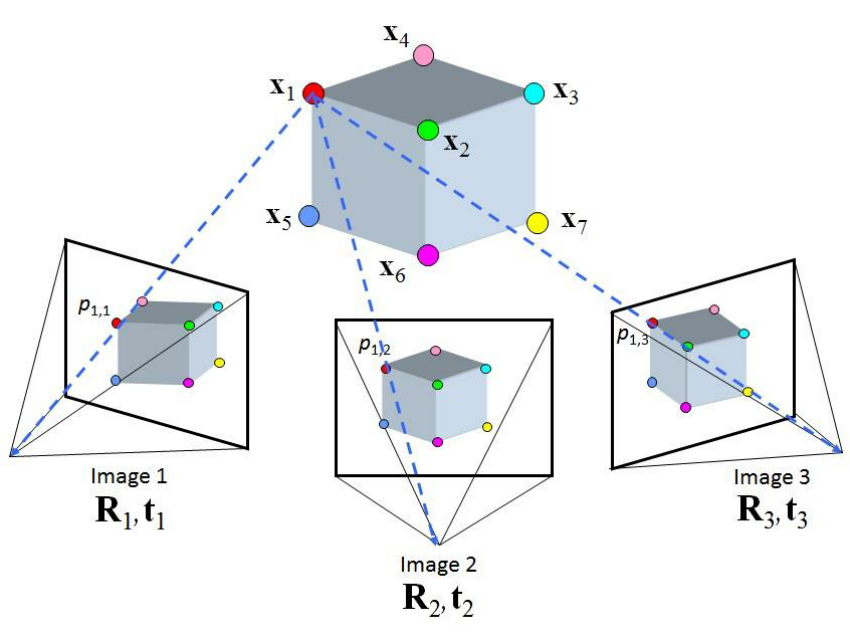
\includegraphics[width=0.5\textwidth]{images/related-work/Structure-from-Motion-SfM-process-is-illustrated-The-structure-in-the.png}
  \caption{Camera pose estimation}
  \label{fig:camera-pose-estimation}
  % https://www.researchgate.net/figure/Structure-from-Motion-SfM-process-is-illustrated-The-structure-in-the_fig2_269327935
\end{figure}

The camera pose estimation (visualized in Figure
\ref{fig:camera-pose-estimation}) starts with an initialization step,
where the initial pair of images and matched features between them
are used to estimate the camera pose. Then, the algorithm proceeds to
the loop (Figure \ref{fig:colmap-pipeline}), where the next image is
registered to the reconstruction and the camera pose is estimated
again (triangulation step). After that the bundle adjustment step is
performed to refine the camera poses and 3D points to be consistent
with the entire dataset with images of a given scene. This
optimization process typically uses the Levenberg-Marquardt algorithm
to minimize reprojection error. This process is repeated for each
subsequent batch of images, updating the camera poses and 3D points.

\subsection{Methods for 3D Reconstruction}

The field of 3D reconstruction encompasses various approaches beyond the basic Structure from Motion pipeline. These methods can be broadly categorized into two groups: sparse reconstruction (like SfM) and dense reconstruction methods.

\subsubsection{Dense Reconstruction Methods}

While SfM provides camera poses and a sparse point cloud, dense reconstruction methods aim to create a complete 3D model with detailed surface information. Notable methods include:

\begin{enumerate}
  \item \textbf{Multi-View Stereo (MVS)}: After obtaining camera poses through SfM, MVS algorithms like PMVS \cite{pmvs} generate dense point clouds by matching pixels across multiple images.

  \item \textbf{Depth Map Fusion}: Methods such as COLMAP's MVS pipeline estimate per-image depth maps and then fuse them into a consistent 3D model.

  \item \textbf{Neural Radiance Fields (NeRF)} \cite{nerf}: A more recent approach that represents scenes as continuous 5D functions (spatial location and viewing direction) encoded in neural networks. NeRF takes camera poses from SfM as input and uses ray tracing to synthesize novel views with remarkable detail and view consistency.
\end{enumerate}

\subsubsection{Learning-based Reconstruction}

Recent approaches leverage deep learning for 3D reconstruction, often using SfM-derived data for supervision or initialization:

\begin{enumerate}
  \item \textbf{Learned MVS}: Methods like MVSNet \cite{mvsnet} use convolutional neural networks to learn the depth estimation process directly from images and camera parameters.

  \item \textbf{Single-view Reconstruction}: Networks like Mesh R-CNN \cite{meshrcnn} can estimate 3D structure from a single image by leveraging prior knowledge learned from large datasets.
\end{enumerate}

\subsection{Limitations of 3D Reconstruction}

Structure from Motion is a powerful tool for 3D reconstruction, demonstrating high effectiveness across a variety of scenarios. However, it encounters significant challenges. These include dealing with textureless surfaces, reflective materials, and the computational complexity of processing high-resolution images. Most importantly in the context of this thesis, it struggles with sparse input scenarios, such as those involving a single image or only a few images.

Traditional 3D reconstruction methods like SfM and MVS typically require a dense collection of images with sufficient overlap to establish accurate feature correspondences and camera pose estimations. When faced with limited input views—particularly in the extreme case of a single image—these methods often fail to generate complete and accurate 3D representations. The quality of reconstruction degrades significantly due to:

\begin{enumerate}
  \item \textbf{Geometric ambiguity}: A single image or sparse set of images provides incomplete information about occluded regions and depth, leading to ambiguous geometry.

  \item \textbf{Feature matching limitations}: Fewer images means fewer opportunities to establish reliable feature correspondences across different viewpoints.

  \item \textbf{Inability to triangulate}: Robust triangulation requires features to be visible from multiple viewpoints, which is not possible with very limited inputs.

  \item \textbf{View-dependent effects}: Materials with specular reflections or varying appearance based on viewpoint cannot be accurately modeled without multiple observations.
\end{enumerate}

These limitations have motivated the development of generative approaches to novel view synthesis, particularly using diffusion models trained on large datasets of rendered images of 3D models. Instead of explicitly reconstructing geometry, these methods leverage the power of deep learning to hallucinate plausible views from unseen perspectives.

\begin{figure}[h]
  \centering
  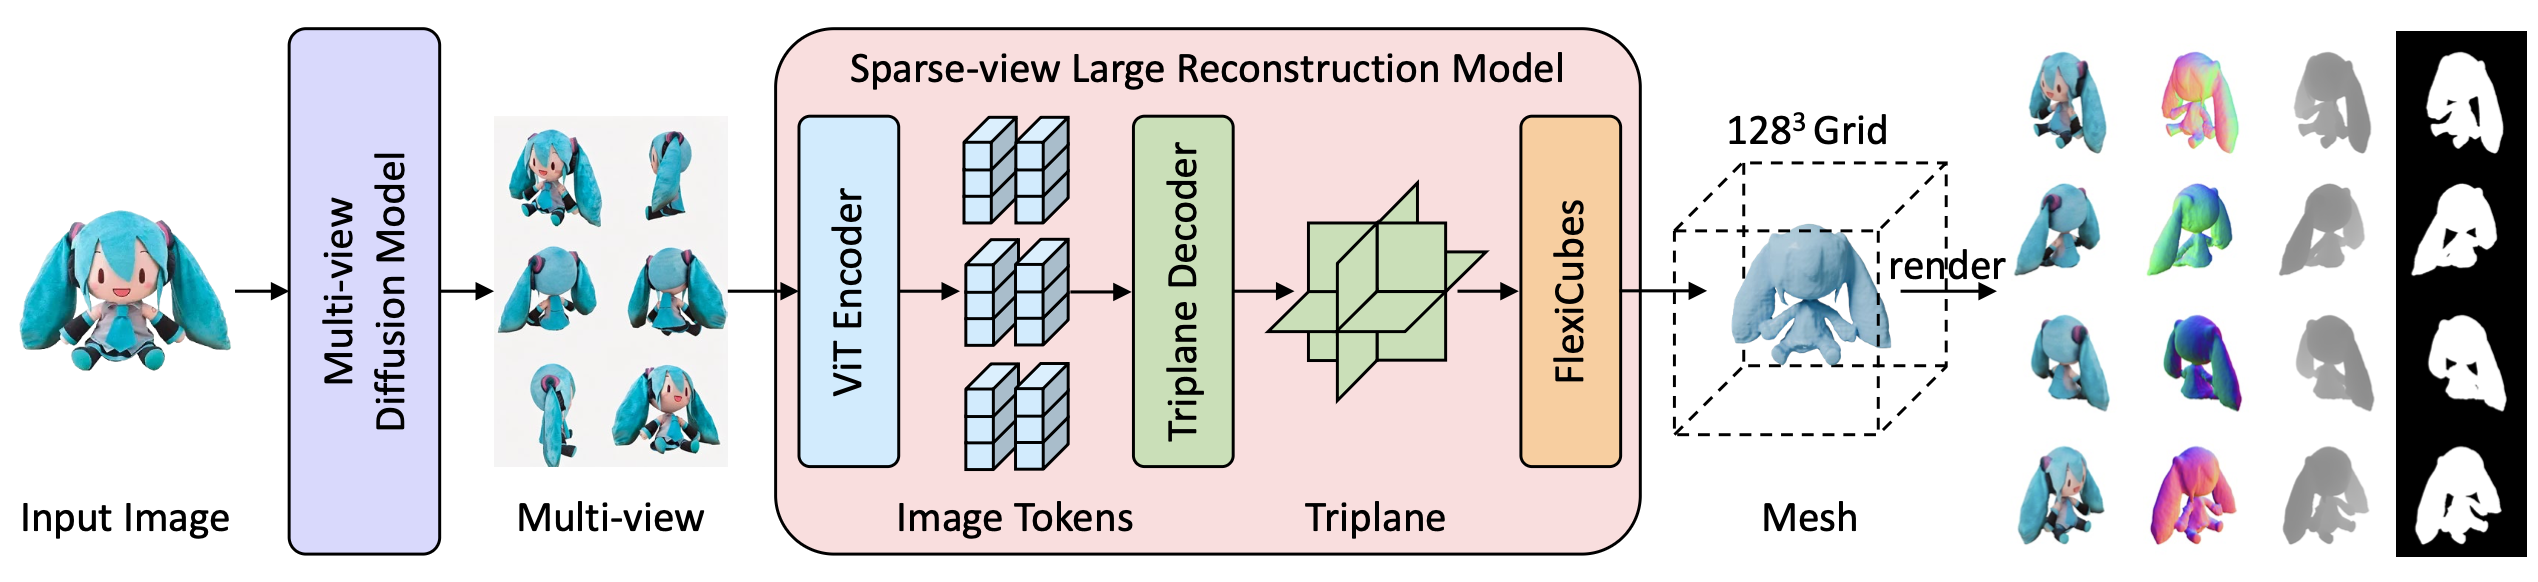
\includegraphics[width=\textwidth]{images/related-work/instantmesh.png}
  \caption{InstantMesh}
  \label{fig:instantmesh}
\end{figure}

Modern approaches of 3D object generation, such as InstantMesh \cite{instantmesh}, leverage these diffusion models to generate multiple consistent views of an object from minimal input (a single image or even a text prompt). This novel view synthesis is the first step in a pipeline \ref{fig:instantmesh} that can be used to create a 3D model of the object, and it is this particular step that forms the central focus of this thesis.

\section{Deep Generative Models for Image Synthesis}\label{sec:text-to-image}

The development of deep learning methods has led to remarkable progress in generative modeling, enabling the synthesis of highly realistic and diverse images. Among the various approaches, Generative Adversarial Networks (GANs), Variational Autoencoders (VAEs), and Diffusion Models have emerged as the most prominent. While GANs and VAEs have laid significant groundwork and continue to be influential, this section will primarily focus on diffusion models, given their state-of-the-art performance in image quality and controllability, and their direct relevance to the multi-view synthesis tasks explored in this thesis.

\subsection{Generative Adversarial Networks (GANs) and Variational Autoencoders (VAEs)}

Generative Adversarial Networks (GANs) \cite{gan} consist of two neural networks, a generator and a discriminator, trained in a competitive setting. The generator aims to produce realistic images, while the discriminator tries to distinguish between real images from the training dataset and fake images produced by the generator. Through this adversarial process, the generator learns to create increasingly plausible images. GANs are known for generating sharp images but often suffer from training instability.

Variational Autoencoders (VAEs) \cite{vae} are another class of generative models that learn a probabilistic mapping from a high-dimensional data space (e.g., images) to a lower-dimensional latent space, and then back to the data space. A VAE consists of an encoder that compresses the input data into a latent representation (typically a mean and variance defining a Gaussian distribution) and a decoder that reconstructs the data from samples drawn from this latent distribution. They are trained to maximize the evidence lower bound (ELBO), which involves a reconstruction loss and a regularization term (KL divergence) that encourages the latent space to be smooth and well-behaved. VAEs generally offer more stable training than GANs and can learn a meaningful latent space, but often produce slightly blurrier images. VAEs play a crucial role in the architecture of Latent Diffusion Models.

\subsection{Diffusion Models}
Diffusion models have recently become the dominant paradigm in high-fidelity image generation. They are inspired by non-equilibrium thermodynamics, specifically diffusion processes.

\subsubsection{Core Concept: The Diffusion Process}
The core idea behind diffusion models involves two processes: a forward (or diffusion) process and a reverse (or denoising) process.
In the \textbf{forward process}, a known image $x_0$ from the dataset is gradually perturbed by adding small amounts of Gaussian noise over a sequence of $T$ steps. This process progressively corrupts the image until, at step $T$, it becomes indistinguishable from pure isotropic Gaussian noise. The parameters of this noising process are fixed.

The \textbf{reverse process} aims to learn to reverse this noising. Starting from pure noise (equivalent to $x_T$), a neural network is trained to gradually denoise the signal, step-by-step, eventually producing a realistic image (an approximation of $x_0$). This learned denoising process is what allows the model to generate new images. Figure \ref{fig:diffusion-process} illustrates this concept.

\begin{figure}[h]
  \centering
  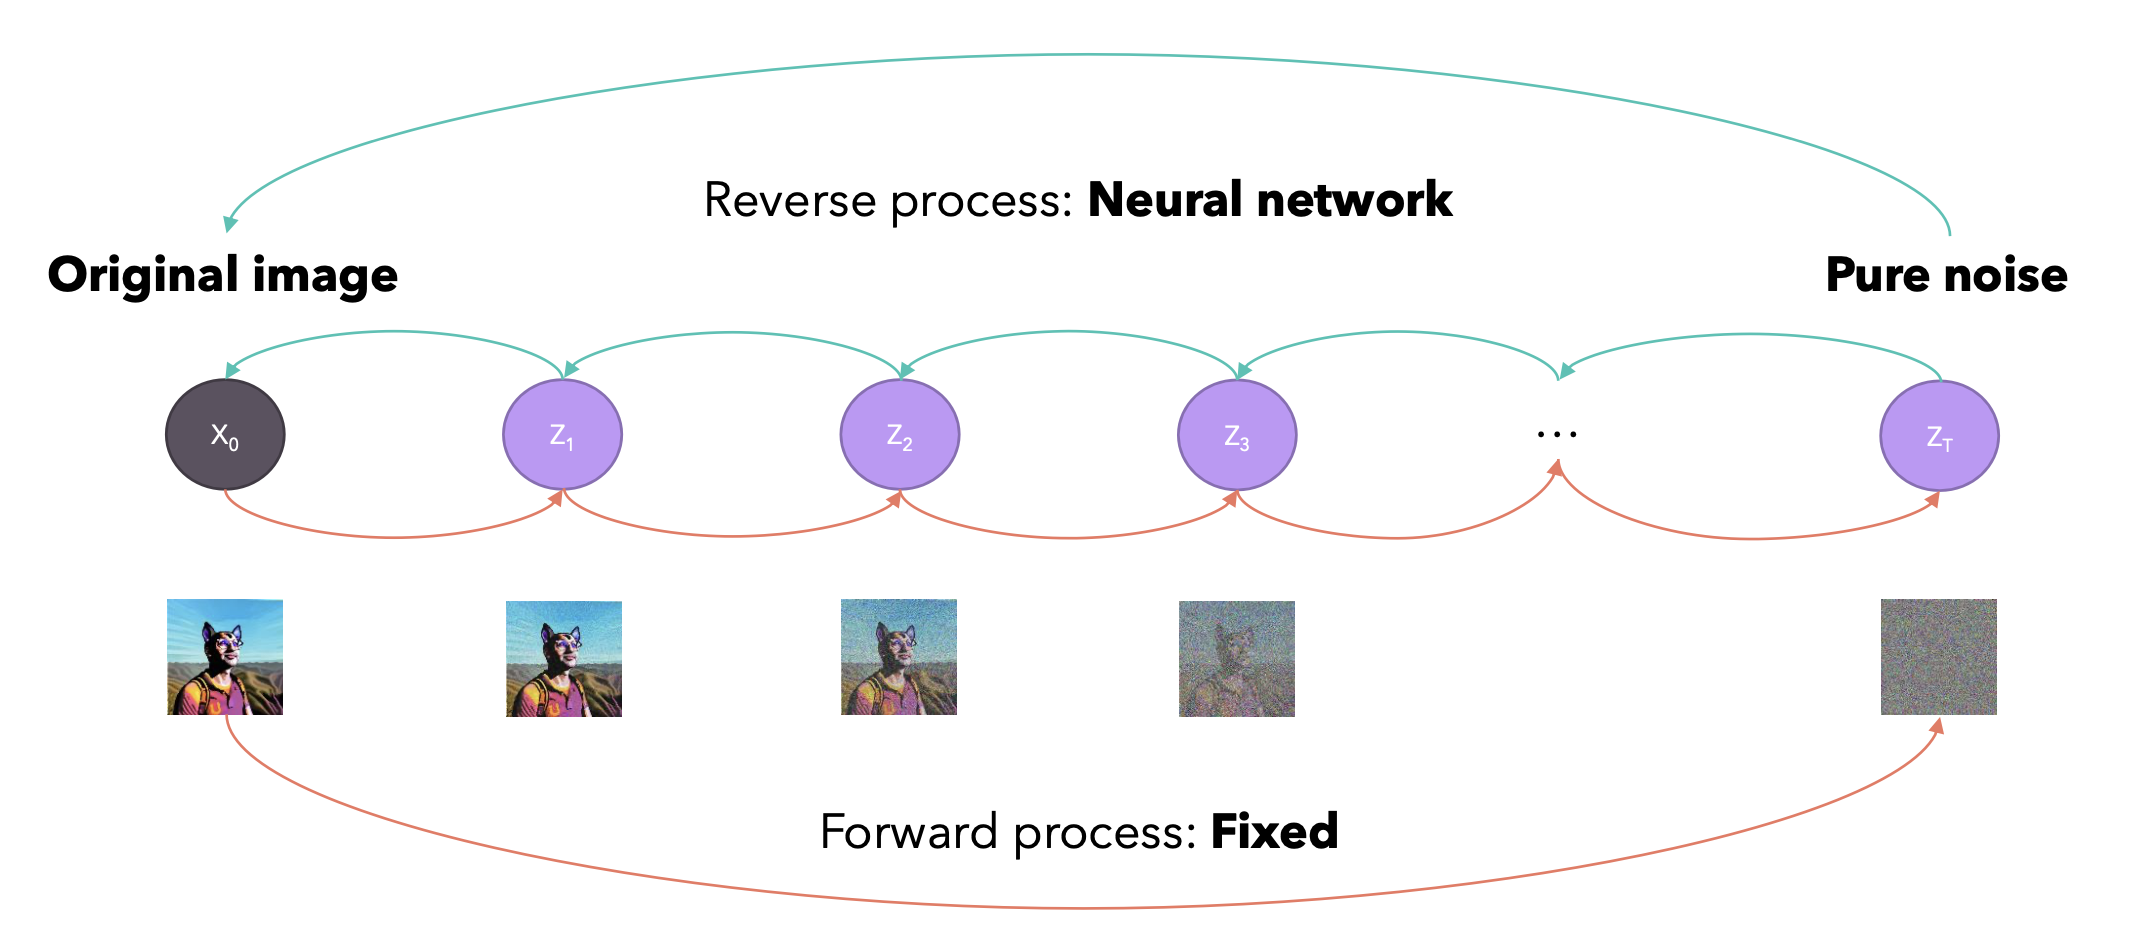
\includegraphics[width=0.8\textwidth]{images/related-work/diffusion-process.png}
  \caption{The forward (noising) and reverse (denoising/generation) stages of a diffusion model. The forward process gradually adds noise to an image until it becomes pure noise. The reverse process learned by a neural net to denoise, step-by-step, to generate an image from noise.}
  \label{fig:diffusion-process}
\end{figure}

\subsubsection{The U-Net Architecture}
The neural network responsible for predicting the noise (or the denoised image) at each step in the reverse process is typically a U-Net architecture \cite{unet}. The U-Net, originally developed for biomedical image segmentation, features an encoder-decoder structure with skip (residual) connections. The encoder path progressively downsamples the input, capturing contextual information, while the decoder path progressively upsamples, localizing information. The skip connections concatenate features from the encoder to corresponding layers in the decoder, allowing the network to combine high-level semantic information with low-level detail, which is crucial for accurately predicting the noise and preserving image fidelity during the denoising steps.

\subsubsection{Training Objective and Loss Function}
The training objective of the diffusion model is to learn the conditional probability distribution $p_\theta(x_{t-1}|x_t)$, which represents the probability of the previous, less noisy state $x_{t-1}$ given the current noisy state $x_t$. In practice, this is often simplified to training the U-Net to predict the noise $\epsilon$ that was added to an image $x_0$ to produce $x_t$ at a given timestep $t$. The loss function is typically the Mean Squared Error (MSE) between the true added noise $\epsilon$ and the noise $\epsilon_\theta(x_t, t)$ predicted by the U-Net:
\[ L = \mathbb{E}_{t \sim [1, T], x_0 \sim q(x_0), \epsilon \sim \mathcal{N}(0, I)} [\|\epsilon - \epsilon_\theta(x_t, t)\|^2] \]
where $x_t = \sqrt{\bar{\alpha}_t}x_0 + \sqrt{1-\bar{\alpha}_t}\epsilon$, and $\bar{\alpha}_t$ are parameters from the noise schedule.

\subsubsection{Conditional Generation: Text-to-Image Synthesis}
To guide the image generation process, diffusion models can be conditioned on various inputs, most notably text prompts. This is the foundation of text-to-image synthesis.
A crucial component for text conditioning is a powerful text encoder that can convert textual descriptions into rich numerical representations (embeddings). Contrastive Language-Image Pre-training (CLIP) \cite{clip} is widely used for this purpose. CLIP is trained on a massive dataset of image-text pairs to learn a shared embedding space where semantically similar images and texts are close together.

The text embeddings from CLIP are then integrated into the U-Net, typically using cross-attention mechanisms. In these layers, the image representation at an intermediate layer of the U-Net queries the text embedding, allowing the model to align parts of the image with relevant words or phrases in the prompt. This enables fine-grained control over the generated image content based on the textual input.

\subsection{Latent Diffusion Models (LDMs)}\label{ssec:ldm}
While standard diffusion models operate directly in the pixel space of images, this can be computationally very expensive, especially for high-resolution images, as the U-Net needs to process large tensors. Latent Diffusion Models (LDMs) \cite{stablediffusion}, such as Stable Diffusion, address this challenge by performing the diffusion and denoising process in a lower-dimensional latent space.

LDMs employ a pre-trained autoencoder, typically a VAE. The VAE's encoder first compresses a high-resolution image from pixel space into a compact latent representation. The diffusion process (both forward and reverse) then occurs entirely within this latent space. Once the reverse denoising process generates a target latent representation from noise, the VAE's decoder maps this latent representation back into the high-resolution pixel space to produce the final image. Figure \ref{fig:ldm-architecture} depicts the architecture of an LDM.

\begin{figure}[h]
  \centering
  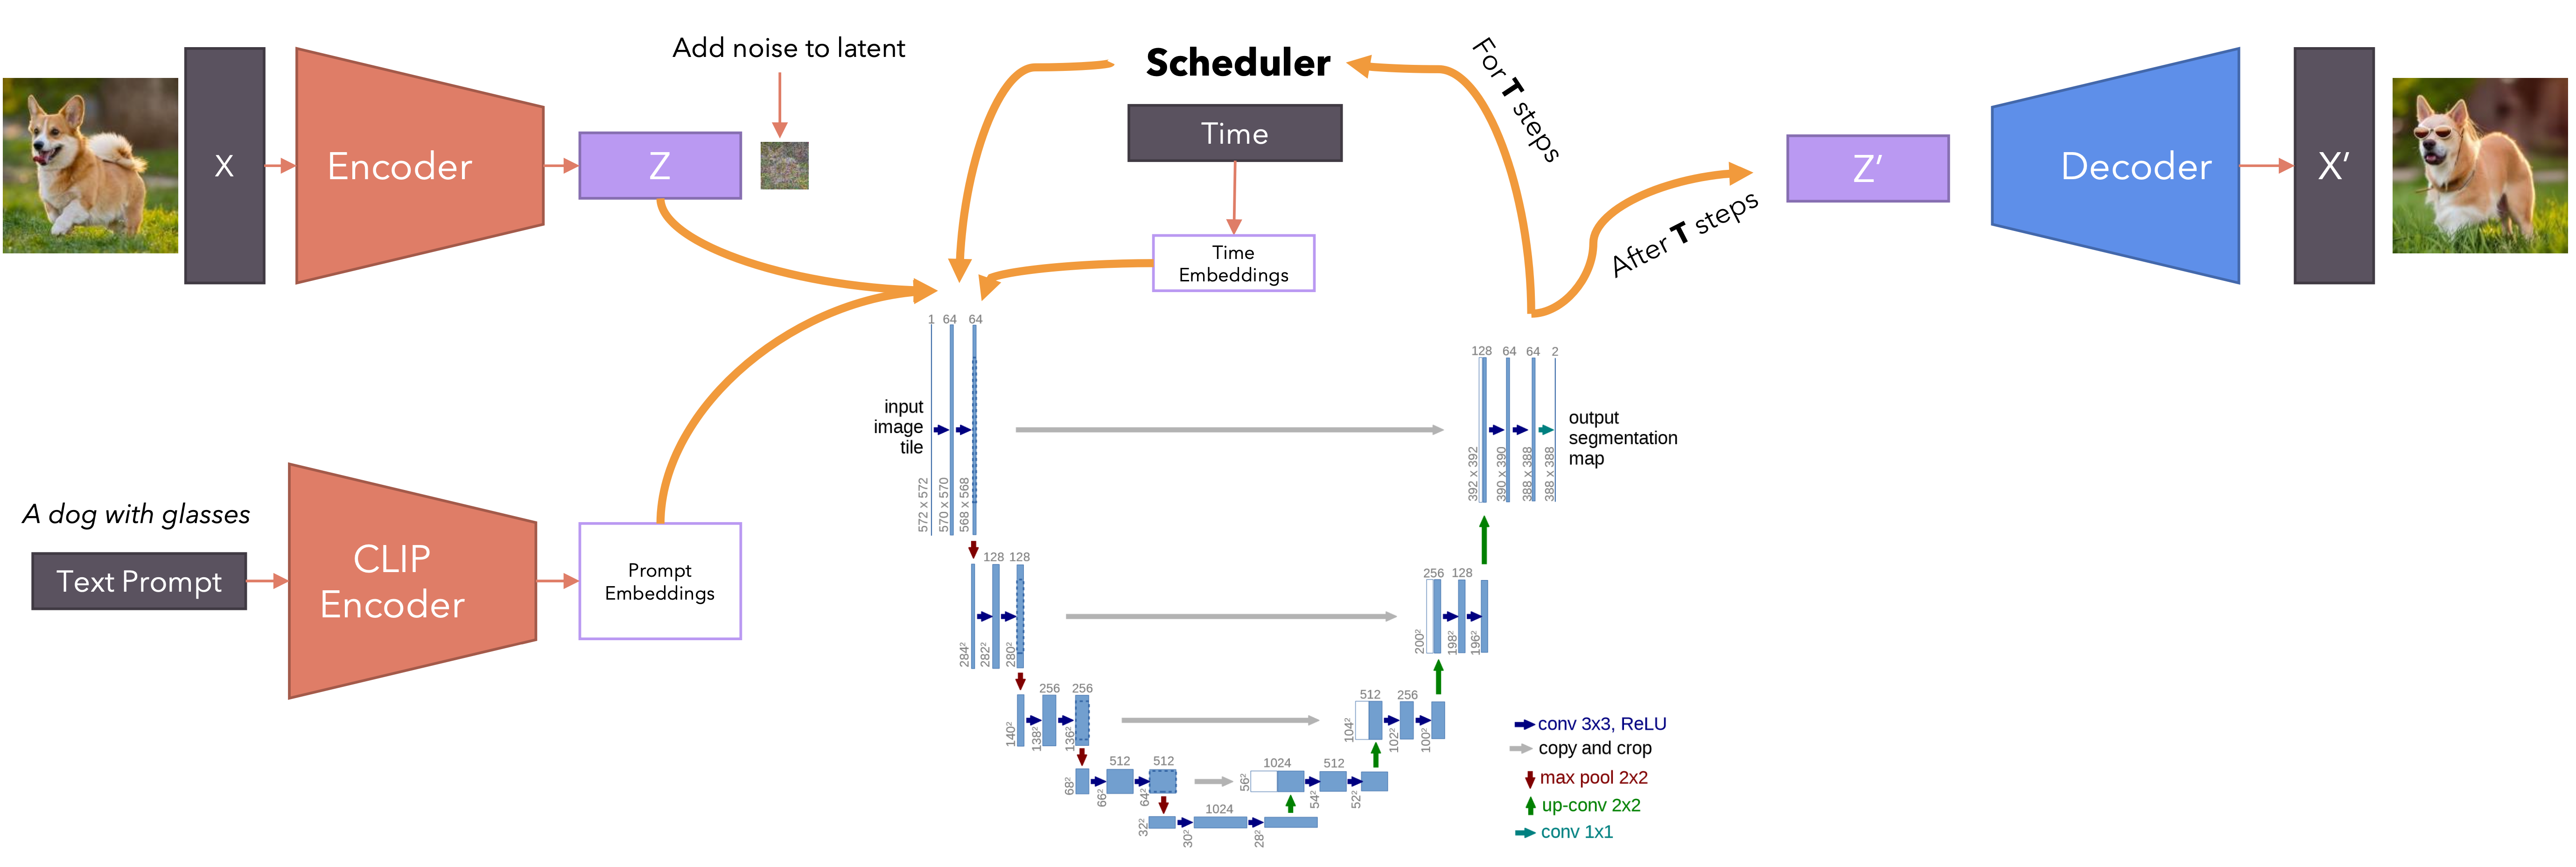
\includegraphics[width=\textwidth]{images/related-work/LDM-detailed.png}
  \caption{Architecture of a Latent Diffusion Model (LDM). An image is first encoded into a latent space by a VAE encoder. The diffusion process (noising and denoising via U-Net) occurs in this latent space. The generated latent is then decoded back to pixel space by the VAE decoder. Conditioning, such as text embeddings from CLIP, is incorporated into the U-Net.}
  \label{fig:ldm-architecture}
\end{figure}

By working in a compressed latent space, LDMs significantly reduce the computational burden during training and inference compared to pixel-space diffusion models. This makes it feasible to train powerful models on massive datasets and generate high-resolution images more efficiently, without a substantial loss in quality. The VAE ensures that the latent space is perceptually equivalent to the pixel space, and the diffusion model learns to generate high-quality latents within this space.

\section{Conditioning Diffusion Models for Enhanced Control and New
Tasks}\label{sec:conditioning-diffusion}

\subsection{Diverse Conditioning Signals}

\subsection{Camera Parameter Encoding for 3D Awareness}

\subsection{Lightweight Adaptation}

To address the limitations of full fine-tuning approaches, recent
works have explored adapter-based methods that allow for more
efficient adaptation of pre-trained models to specific tasks while
preserving their original capabilities.

Adapters are lightweight modules that can be inserted into
pre-trained models to adapt them to new tasks without modifying the
original network parameters. This approach has gained popularity in
natural language processing and has also been applied to diffusion
models for various image generation tasks.

ControlNet \cite{controlnet} introduced a method to add spatial
conditioning to text-to-image diffusion models by training additional
control modules that are connected to the original UNet backbone.
This approach allows for precise control over the generated images
while preserving the original model's capabilities.

Similarly, T2I-Adapter \cite{t2iadapter} proposed a more modular
approach where adapters are trained separately and can be combined to
provide multiple forms of control simultaneously. These methods have
demonstrated the effectiveness of adapter-based approaches for
controlled image generation.

\section{Diffusion-based Multi-View Image
Generation}\label{sec:multi-view-diffusion}

\subsection{Single Reference Image Novel View Synthesis}

Zero-1-to-3 \cite{zero1to3} pioneered the approach of conditioning
diffusion models on both a reference image and camera pose
information to generate novel views. This method demonstrated the
potential of leveraging pre-trained text-to-image models for novel
view synthesis without requiring explicit 3D reconstruction. However,
it often struggles with maintaining geometric consistency across
generated views.

\subsection{Coherent Multi-View Generation Architectures}
% Camera encoding

To address the limitations of single-view approaches, several works
have focused on developing multi-view diffusion models that can
generate multiple consistent views simultaneously.

MVDream \cite{mvdream} extends the self-attention mechanism in
diffusion models to operate across multiple views, enabling the
generation of 3D-consistent images. By jointly modeling multiple
views, this approach significantly improves geometric consistency
compared to methods that generate each view independently.

Similarly, ViewCrafter \cite{viewcrafter} combines video latent
diffusion models \cite{videolatentdiffusion} with 3D point cloud
priors to generate high-fidelity and consistent novel views. By
leveraging the explicit 3D information provided by point clouds and
the generative capabilities of video diffusion models, ViewCrafter
achieves precise control of camera poses and generates high-quality novel views.

CAT3D \cite{cat3d} takes a different approach by simulating a
real-world capture process with a multi-view diffusion model. Given
one or three input images and a set of target novel viewpoints, this
model generates highly consistent novel views that can be used as
input to robust 3D reconstruction techniques.

While these multi-view diffusion models have shown impressive
results, they typically require full fine-tuning of pre-trained
text-to-image models, which is computationally expensive and may lead
to degradation in image quality due to the scarcity of high-quality 3D data.

\subsection{Specialized Multi-View Adapters}

Building upon the success of adapter mechanisms, MV-Adapter
\cite{mvadapter} introduced the first adapter-based solution for
multi-view image generation. Unlike previous approaches that make
invasive modifications to pre-trained text-to-image models and
require full fine-tuning, MV-Adapter enhances these models with a
plug-and-play adapter that preserves the original network structure
and feature space.

MV-Adapter employs a decoupled attention mechanism, where the
original spatial self-attention layers are retained, and new
multi-view attention layers are created by duplicating the structure
and weights of the original layers. These layers are organized in a
parallel architecture, allowing the adapter to inherit the powerful
priors of the pre-trained self-attention layers while efficiently
learning geometric knowledge.

Additionally, MV-Adapter introduces a unified condition encoder that
seamlessly integrates camera parameters and geometric information,
facilitating applications such as text and image-based 3D generation
and texturing. By updating fewer parameters, MV-Adapter enables
efficient training and preserves the prior knowledge embedded in
pre-trained models, mitigating overfitting risks.

problems of the current MVD:
- inconsistant lighting
- poor geometric consistency
- big model training requirements